% =====================================================================
%  CS 6330 - Introduction to Data Science
%  Homework 3: YouTube comments, word clouds, comparison
%  Author: Taek Lim
%
%  Build (from hw3/report/):  latexmk -C && latexmk -xelatex hw3_taeklim_report.tex
%  XeLaTeX, not pdfLaTeX: video A's title and the non-English term tables hold Hangul,
%  Thai and kana (owner, 2026-10-04).
%
%  Every number comes from a generated file: tables/counts.tex (macros) and the other
%  tables/*.tex. Run hw3/code/p4_report_tables.py to rebuild them. Figure paths are
%  relative to this file: ../figures/*.png
% =====================================================================
\documentclass[11pt]{article}

\usepackage[letterpaper,margin=0.75in]{geometry}
\usepackage{fontspec}     % body font: the default Latin Modern Roman (= hw2's Computer Modern)
\usepackage{amsmath}
\usepackage{booktabs}     % \toprule \midrule \bottomrule
\usepackage{tabularx}
\usepackage{graphicx}
\usepackage{float}        % [H]
\usepackage{caption}
\usepackage{xcolor}
\usepackage[hidelinks]{hyperref}
\usepackage{enumitem}

% Font that draws Hangul, Thai, kana and Cyrillic. The generated tables wrap such cells in
% {\unifont ...}; the report text itself is Latin.
\newfontfamily\unifont{Arial Unicode MS}

\captionsetup{font=small, labelfont=bf}
\setlength{\parindent}{0pt}
\setlength{\parskip}{0.5em}

\setlist{leftmargin=0pt, itemindent=*, labelsep=0.5em}
\definecolor{prompt}{HTML}{1F4E9A}
\newcommand{\prompt}[1]{\textcolor{prompt}{#1}}
\setlist[itemize,1]{label=\prompt{-}}

% Placeholder for text only the author can give (book.md principle 13).
\newcommand{\todo}[1]{\textcolor{red}{\textbf{[TODO: #1]}}}

% One word cloud per float: \cloudfig{file}{label}{caption}.
\newcommand{\cloudfig}[3]{%
  \begin{figure}[H]
    \centering
    \includegraphics[width=\linewidth,height=0.42\textheight,keepaspectratio]{../figures/#1.png}
    \caption{#3}\label{fig:#2}
  \end{figure}}


% Generated table bodies end with a row break. LaTeX's \input hooks put tokens after the file,
% so \bottomrule would be misplaced; the primitive \@@input has no hook.
\makeatletter
\newcommand{\gentable}[1]{\@@input #1 }
\makeatother

% Comment counts and video statistics (generated).
\newcommand{\nEnVideoA}{1,000}
\newcommand{\nNonEnVideoA}{965}
\newcommand{\nMixedVideoA}{1,965}
\newcommand{\nFetchedVideoA}{1,965}
\newcommand{\nViewsVideoA}{2,146,874,108}
\newcommand{\nLikesVideoA}{39,661,294}
\newcommand{\nCommentsVideoA}{15,898,150}
\newcommand{\nEnVideoB}{1,000}
\newcommand{\nNonEnVideoB}{1,127}
\newcommand{\nMixedVideoB}{2,127}
\newcommand{\nFetchedVideoB}{2,127}
\newcommand{\nViewsVideoB}{2,243,728,665}
\newcommand{\nLikesVideoB}{26,742,200}
\newcommand{\nCommentsVideoB}{2,500,163}


\begin{document}

\hfill Taek Lim \quad CS 6330 Homework 3: YouTube Comments and Word Clouds

\bigskip
\textbf{Tooling.} Python 3 / pandas / lingua (language detection) / wordcloud / matplotlib;
every number and table body is generated from saved data files, none typed by hand; analysis
code and write-up drafted with Claude Code. The code is in the repository
\url{https://github.com/intothedeep/mscs_utrgv_cs6330_intro_2_ds}, folder \texttt{hw3/code}.

% =====================================================================
\section{Data collection}

I compare two music videos: BTS \emph{Dynamite} (video A) and BLACKPINK \emph{Kill This Love}
(video B). The data comes from the YouTube Data API through a YouTube Data API v3 key from my
own Google Cloud project; the key is not shown. The steps are as follows:
Table~\ref{tab:pipeline} puts the assignment's R functions next to the Python scripts that do the same step.

\begin{table}[H]
\centering
\caption{Pipeline: the R step of the assignment script and the Python step that replaces it.}\label{tab:pipeline}
\footnotesize
\begin{tabularx}{\linewidth}{@{}l>{\raggedright\arraybackslash}p{0.22\linewidth}>{\raggedright\arraybackslash}p{0.27\linewidth}>{\raggedright\arraybackslash}X@{}}
  \toprule
  Step & R function & Python function & Output file \\
  \midrule
  1. Stats and details & \texttt{get\_stats}, \texttt{get\_video\_details} & \texttt{p1\_collect.fetch\_video} & \texttt{data/videos.csv} \\
  \midrule
  2. Comments & \texttt{get\_comment\_threads}, \texttt{write.csv} & \texttt{p1\_collect.fetch\_comments} & \texttt{data/comments\_<label>\_all.csv}, \texttt{data/comments\_<label>.csv} \\
  \midrule
  3. Terms & \texttt{Corpus}, \texttt{DocumentTermMatrix}, \texttt{colSums} & \texttt{common.clean\_terms}, \texttt{common.count\_terms} & \texttt{data/terms\_<label>\_<version>.csv} \\
  \midrule
  4. Word cloud & \texttt{wordcloud} & \texttt{p2\_wordcloud.make\_cloud} & \texttt{figures/wordcloud\_*.png} \\
  \midrule
  5. Comparison & none & \texttt{p3\_compare.py} & \texttt{data/compare\_videos.csv}, \texttt{data/compare\_terms.csv} \\
  \bottomrule
\end{tabularx}
\end{table}

\subsection{Videos and statistics}

Table~\ref{tab:stats} gives the details and statistics of both videos as of 2026-10-04. The
comment count is the total YouTube reports; the script fetched \nFetchedVideoA{} top-level
comments of video A and \nFetchedVideoB{} of video B, and kept \nEnVideoA{} English comments of each
for the English word clouds.

\begin{table}[H]
\centering
\caption{Video details and statistics (\texttt{data/videos.csv}).}\label{tab:stats}
\small
\begin{tabular}{@{}lp{0.32\linewidth}p{0.32\linewidth}@{}}
  \toprule
  & Video A & Video B \\
  \midrule
  \gentable{tables/stats.tex}
  \bottomrule
\end{tabular}
\end{table}

\subsection{Sample}

The script reads the top-level comments by relevance order first, then newest first, until
\nEnVideoA{} comments are English (video A) or \nEnVideoB{} (video B), or a page limit is reached. Each
row keeps its order. Table~\ref{tab:sample} counts the fetched comments by order and
detected language.

\begin{table}[H]
\centering
\caption{Sample composition by fetch order and detected language (\texttt{data/sample\_composition.csv}). ``Time'' is newest first. ``No language'' means emoji or links only.}\label{tab:sample}
\small
\begin{tabular}{@{}llrrrr@{}}
  \toprule
  Video & Order & English & \shortstack{Non-English\\(language found)} & No language & Total \\
  \midrule
  \gentable{tables/sample.tex}
  \bottomrule
\end{tabular}
\end{table}

\subsection{First comments}

Table~\ref{tab:first_a} and Table~\ref{tab:first_b} show the first five fetched comments of
each video, in relevance order. The author handle and the comment ID are dropped, every
@mention is replaced by \texttt{@user}, emoji are removed, and long text is cut with
``\dots''. Table~\ref{tab:first_a} and Table~\ref{tab:first_b} stand in for the screenshot of the data.

\begin{table}[H]
\centering
\caption{Video A, first five fetched comments (relevance order). ``Likes'' and ``replies'' are the comment's counts; ``lang'' is the detected language.}\label{tab:first_a}
\footnotesize
\begin{tabular}{@{}rlrrrlp{0.45\linewidth}@{}}
  \toprule
  \# & Order & Published & Likes & Replies & Lang & Comment \\
  \midrule
  \gentable{tables/first_comments_video_a.tex}
  \bottomrule
\end{tabular}
\end{table}

\begin{table}[H]
\centering
\caption{Video B, first five fetched comments (relevance order). Columns as in Table~\ref{tab:first_a}.}\label{tab:first_b}
\footnotesize
\begin{tabular}{@{}rlrrrlp{0.45\linewidth}@{}}
  \toprule
  \# & Order & Published & Likes & Replies & Lang & Comment \\
  \midrule
  \gentable{tables/first_comments_video_b.tex}
  \bottomrule
\end{tabular}
\end{table}

% =====================================================================
\section{Text cleaning and language split}

Each comment gets a language label from the \texttt{lingua} detector, restricted to 20
candidate languages (\texttt{common.LANGUAGES}). With all languages the detector labelled short
English comments as Sotho or Tswana, so the candidate list is cut. URLs and @mentions are
removed before detection. A comment with no words left gets the empty label and goes to the
non-English group.

The word clouds use three versions of the comments of each video:
\begin{itemize}
  \item \textbf{English:} comments detected as English (the first \nEnVideoA{} of video A, the first \nEnVideoB{} of video B).
  \item \textbf{Non-English:} every other fetched comment, including those with no language.
  \item \textbf{Mixed:} all fetched comments, English and non-English together.
\end{itemize}

Table~\ref{tab:cleaning} lists the steps from a comment to its terms, as in
\texttt{common.clean\_terms}.

\begin{table}[H]
\centering
\caption{Cleaning steps from comment to terms.}\label{tab:cleaning}
\small
\begin{tabularx}{\linewidth}{@{}>{\raggedright\arraybackslash}p{0.03\linewidth}>{\raggedright\arraybackslash}p{0.2\linewidth}>{\raggedright\arraybackslash}X>{\raggedright\arraybackslash}p{0.33\linewidth}@{}}
  \toprule
  \# & Step & What it does & Why (tm equivalent) \\
  \midrule
  1 & Language & Detect the language (above) before any cleaning. & Gives the English, non-English and mixed versions. \\
  \midrule
  2 & Lowercase & Turn every letter to lowercase. & \texttt{tm}-style cleaning. \\
  \midrule
  3 & Drop symbols & Drop punctuation, numbers and emoji; keep letters of every script. & As \texttt{tm} for punctuation and numbers. Emoji are dropped because no word cloud font draws them. Non-Latin words stay, so the non-English and mixed clouds have them. \\
  \midrule
  4 & Stopwords & Drop the \texttt{tm} English stopwords. & English stopwords only. \\
  \midrule
  5 & Short words & Drop words under 3 letters. & \texttt{tm}'s default \texttt{wordLengths = c(3, Inf)}. \\
  \midrule
  6 & No stemming & Words are not reduced to stems. & The R script loads \texttt{SnowballC} but never calls it. \\
  \midrule
  7 & Cloud & Draw the top 150 words, with a fixed random seed. & The cloud is rebuilt exactly from the term counts. \\
  \bottomrule
\end{tabularx}
\end{table}

% =====================================================================
\section{Video A word clouds}

Figure~\ref{fig:wc_a_en}, Figure~\ref{fig:wc_a_non_en} and Figure~\ref{fig:wc_a_mixed} show
the three clouds of BTS \emph{Dynamite}. Each cloud draws the top 150 terms; word size follows
the term count.

\cloudfig{wordcloud_video_a_en}{wc_a_en}{Video A (BTS \emph{Dynamite}), English comments ($n = \nEnVideoA$).}
\cloudfig{wordcloud_video_a_non_en}{wc_a_non_en}{Video A (BTS \emph{Dynamite}), non-English comments ($n = \nNonEnVideoA$).}
\cloudfig{wordcloud_video_a_mixed}{wc_a_mixed}{Video A (BTS \emph{Dynamite}), mixed: all fetched comments ($n = \nMixedVideoA$).}

% =====================================================================
\section{Video B word clouds}

Figure~\ref{fig:wc_b_en}, Figure~\ref{fig:wc_b_non_en} and Figure~\ref{fig:wc_b_mixed} show
the three clouds of BLACKPINK \emph{Kill This Love}, built the same way as those of video A.

\cloudfig{wordcloud_video_b_en}{wc_b_en}{Video B (BLACKPINK \emph{Kill This Love}), English comments ($n = \nEnVideoB$).}
\cloudfig{wordcloud_video_b_non_en}{wc_b_non_en}{Video B (BLACKPINK \emph{Kill This Love}), non-English comments ($n = \nNonEnVideoB$).}
\cloudfig{wordcloud_video_b_mixed}{wc_b_mixed}{Video B (BLACKPINK \emph{Kill This Love}), mixed: all fetched comments ($n = \nMixedVideoB$).}

% =====================================================================
\section{Comparison}

Figure~\ref{fig:grid} puts all six clouds side by side: one row per video, one column per
version. Table~\ref{tab:engagement} gives the engagement measures,
Table~\ref{tab:top_en}, Table~\ref{tab:top_non_en} and Table~\ref{tab:top_mixed} the ten most
frequent terms of each version, and Table~\ref{tab:shared} the top 30 terms of each version
split into shared and distinctive terms. This section reports results only; the discussion is
in Section~\ref{sec:discussion}.

\begin{figure}[H]
  \centering
  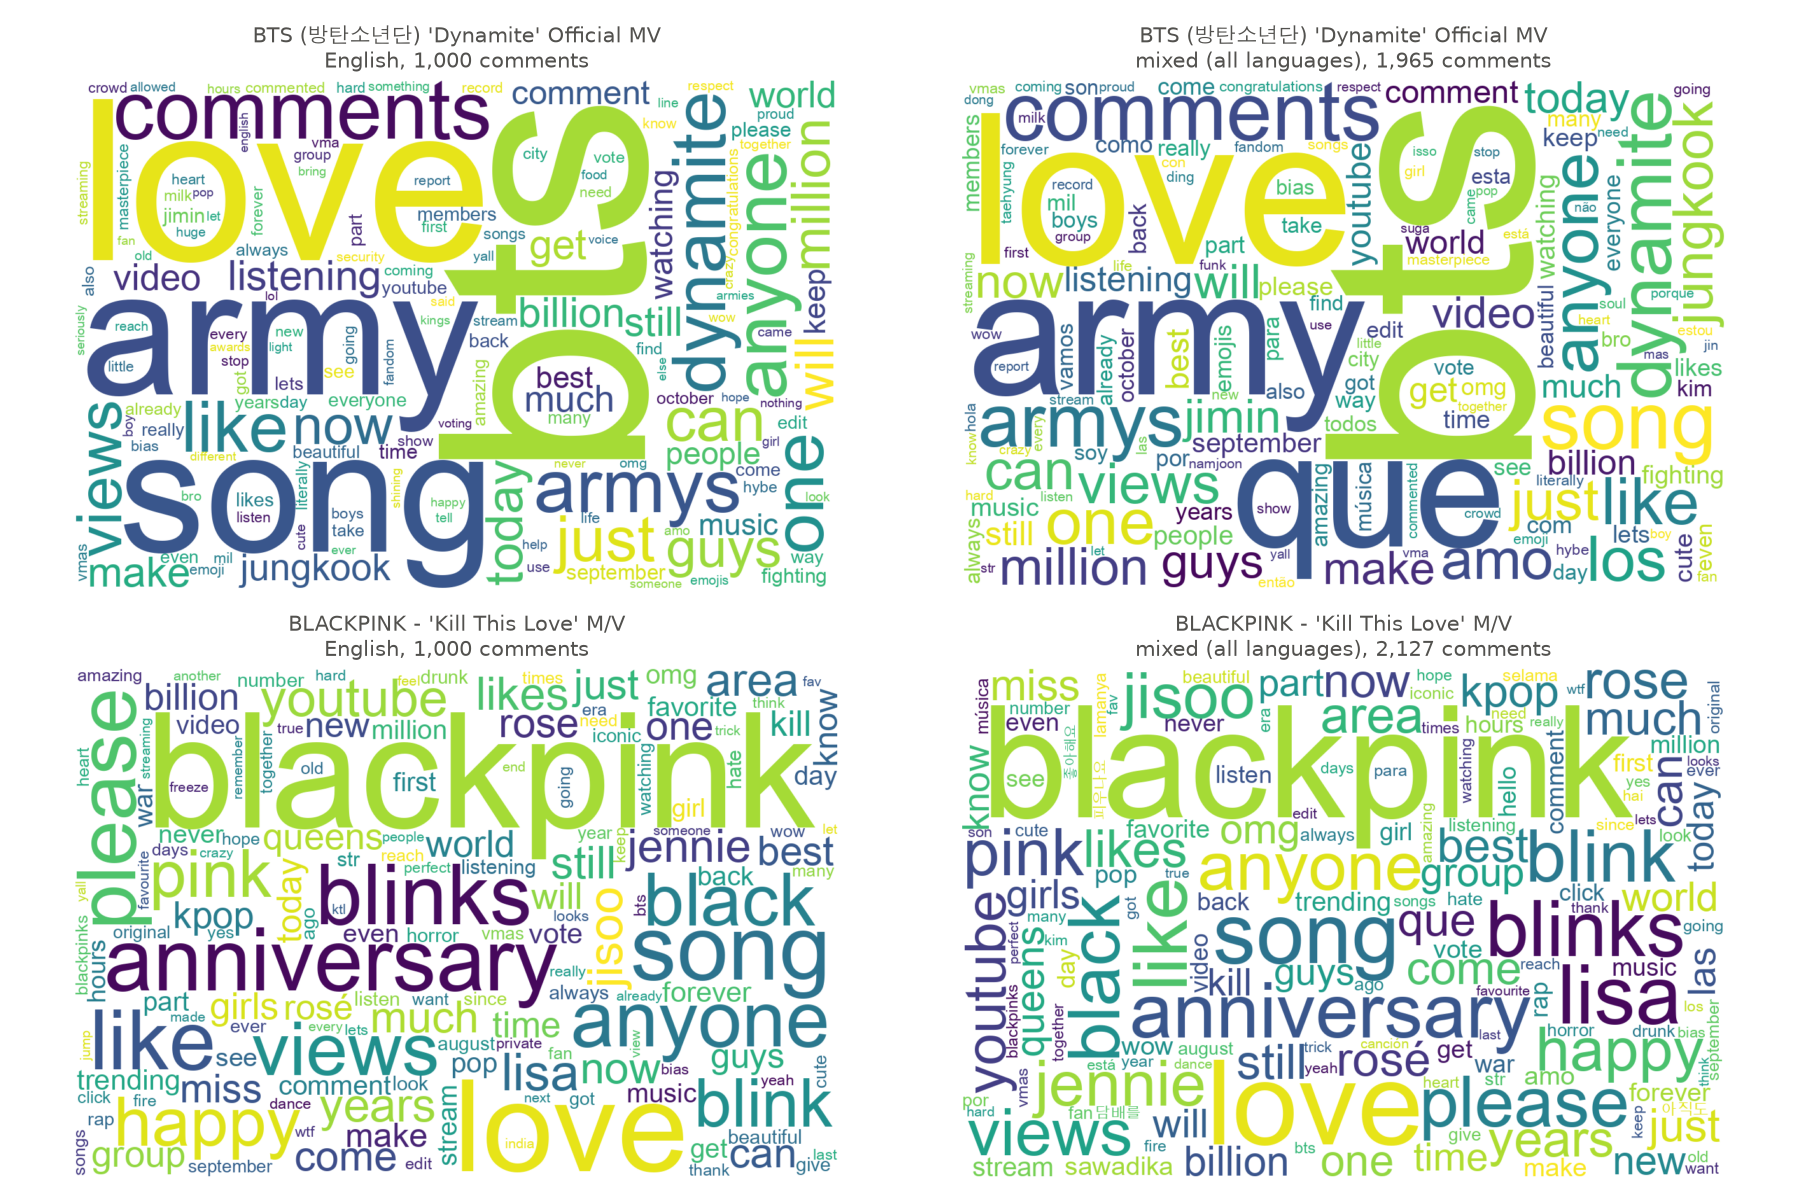
\includegraphics[width=\linewidth,height=0.8\textheight,keepaspectratio]{../figures/wordcloud_grid.png}
  \caption{All six word clouds. Rows: video A (BTS \emph{Dynamite}) and video B (BLACKPINK \emph{Kill This Love}). Columns: English, non-English and mixed comments.}\label{fig:grid}
\end{figure}

\begin{table}[H]
\centering
\caption{Engagement of the two videos (\texttt{data/compare\_videos.csv}). ``Share fetched'' is comments fetched divided by the YouTube comment total; ``share English'' is English comments kept divided by the same total.}\label{tab:engagement}
\small
\begin{tabular}{@{}lrr@{}}
  \toprule
  Measure & Video A & Video B \\
  \midrule
  \gentable{tables/engagement.tex}
  \bottomrule
\end{tabular}
\end{table}

\begin{table}[H]
\centering
\caption{Top 10 terms, English comments, with their counts (\texttt{data/terms\_<label>\_en.csv}).}\label{tab:top_en}
\small
\begin{tabular}{@{}rlrlr@{}}
  \toprule
  Rank & Term A & Count A & Term B & Count B \\
  \midrule
  \gentable{tables/top_terms_en.tex}
  \bottomrule
\end{tabular}
\end{table}

\begin{table}[H]
\centering
\caption{Top 10 terms, non-English comments, with their counts (\texttt{data/terms\_<label>\_non\_en.csv}).}\label{tab:top_non_en}
\small
\begin{tabular}{@{}rlrlr@{}}
  \toprule
  Rank & Term A & Count A & Term B & Count B \\
  \midrule
  \gentable{tables/top_terms_non_en.tex}
  \bottomrule
\end{tabular}
\end{table}

\begin{table}[H]
\centering
\caption{Top 10 terms, mixed comments (all languages), with their counts (\texttt{data/terms\_<label>\_mixed.csv}).}\label{tab:top_mixed}
\small
\begin{tabular}{@{}rlrlr@{}}
  \toprule
  Rank & Term A & Count A & Term B & Count B \\
  \midrule
  \gentable{tables/top_terms_mixed.tex}
  \bottomrule
\end{tabular}
\end{table}

\begin{table}[H]
\centering
\caption{Top 30 terms of each version: in both videos, only in video A, only in video B (\texttt{data/compare\_terms.csv}).}\label{tab:shared}
\scriptsize
\begin{tabular}{@{}p{0.085\linewidth}p{0.27\linewidth}p{0.27\linewidth}p{0.27\linewidth}@{}}
  \toprule
  Version & In both & Only in video A & Only in video B \\
  \midrule
  \gentable{tables/shared_terms.tex}
  \bottomrule
\end{tabular}
\end{table}

% =====================================================================
\section{Discussion}\label{sec:discussion}

The discussion is the author's own comparison and interpretation. It waits for the author's
text; the questions it answers are listed at the end of the report, and it cites Figures~\ref{fig:wc_a_en} to~\ref{fig:grid} and
Tables~\ref{tab:engagement} to~\ref{tab:shared}.

\todo{Owner: discussion text pending; see the open questions at the end of the report (Section~\ref{sec:open_questions}).}

% =====================================================================
\section{Limits of the method}

\begin{itemize}
  \item \textbf{Top-level comments only.} Replies to comments are not fetched; the replies column in Table~\ref{tab:first_a} is only a count.
  \item \textbf{Sample order.} The sample takes relevance order first, then newest first, so it is not a random sample of all comments (Table~\ref{tab:sample}). The YouTube total is far larger than the sample (Table~\ref{tab:stats}).
  \item \textbf{English stopwords only.} Non-English function words stay in the non-English and mixed clouds (Table~\ref{tab:top_non_en}).
  \item \textbf{No stemming, no merging.} Cleaning keeps accents and does not merge variants, so a name written two ways counts as two terms (for example \texttt{rose} and \texttt{rosé} in video B).
  \item \textbf{Language detector errors.} One comment of video A is detected as \texttt{tl} (Tagalog): ``Ommg \dots{} ARMYYY'' (Table~\ref{tab:first_a}, row 5). It is an English-like fan comment, which shows the detector's error on short informal text.
  \item \textbf{Cloud rendering.} Arabic words in a cloud are drawn unjoined, because the cloud tool does no text shaping.
\end{itemize}


% =====================================================================
\section*{Open questions for the author (temporary)}\label{sec:open_questions}

This section is removed before submission.

\begin{enumerate}[label=B\arabic*., leftmargin=2em, itemindent=0pt]
  \item \todo{Owner: The views are close (\nViewsVideoA{} for video A, \nViewsVideoB{} for video B), but the comment totals differ a lot (\nCommentsVideoA{} for video A, \nCommentsVideoB{} for video B). What do you think explains this? (Table~\ref{tab:stats}, Table~\ref{tab:engagement})}
  \item \todo{Owner: Video A ranks \texttt{army}, \texttt{comments}, \texttt{million}, \texttt{views}. Do the comments talk about the song, or about the fandom and its counts? (Table~\ref{tab:top_en}, Table~\ref{tab:shared})}
  \item \todo{Owner: Video B ranks \texttt{anniversary} and \texttt{happy}. What anniversary do you think the comments mean? (Table~\ref{tab:shared})}
  \item \todo{Owner: \texttt{love} ranks second in both. Is it the same meaning in both? (Video B's title holds ``Love''.) (Table~\ref{tab:top_en})}
  \item \todo{Owner: Video B names four members, video A mostly one. What does that say, if anything? (Table~\ref{tab:shared})}
  \item \todo{Owner: Which of the three cloud versions best supports your comparison, and why? (Figures~\ref{fig:wc_a_en} to~\ref{fig:grid})}
  \item \todo{Owner: What does the non-English cloud say about each audience? Is it useful given the stopword limit? (Figure~\ref{fig:wc_a_non_en}, Figure~\ref{fig:wc_b_non_en}, Table~\ref{tab:top_non_en})}
  \item \todo{Owner: Does mixing relevance order and newest-first order change what the clouds show? (Table~\ref{tab:sample})}
  \item \todo{Owner: What is your overall conclusion: how are the two comment sections alike, and how do they differ?}
\end{enumerate}

\end{document}
